% !TeX root=../main.tex
\chapter{پیاده سازی رویکرد گراف مبنا جهت موقعیت‌یابی و کالیبراسیون همزمان برای ربات کابلی خم‌شده}
%\thispagestyle{empty} 
این پایان‌نامه به بررسی دقیق رویکردهای مختلف در حوزه رباتیک برای فرمول‌بندی ریاضی یک مسئله بهینه‌سازی مقید پرداخته است. از تحلیل مزایا و معایب روش‌های مرسوم تا رویکردهای جدید مبتنی بر گراف، روشی جامع برای فرمول‌بندی و حل مسئله بهینه‌سازی کالیبراسیون و مکان‌یابی همزمان ربات‌ها ارائه شده است. در فصل گذشته، عملکرد این روش بر روی یک ربات کابلی مقید که کابل‌های آن به صورت صلب در نظر گرفته شده بود، ارزیابی شد. پس از معرفی فرمول‌بندی سینماتیکی، گراف مربوط به آن ساخته و نتایج پیاده‌سازی بررسی شد. آنچه از ابتدای این پایان‌نامه به عنوان هدفی مهم معرفی گردید، ماژولاریتی و انعطاف‌پذیری روش، با قیدهای متفاوت و گسترده بود. انتخاب ربات کابلی به عنوان مورد مورد مطالعه، نیز به دلیل امکان پیاده‌سازی و ارزیابی همین هدف بوده است.

در این فصل، بدون تغییر در فرمول‌بندی‌های ارائه شده در فصل قبل، به مسئله قیدهای دینامیکی کابل افزوده خواهد شد. علیرغم پیچیدگی این مدل‌ها، حل‌کننده همچنان با دقت و سرعت بالا به نتایج مطلوب دست خواهد یافت. تاکنون تحقیقات بسیاری بر مدل‌سازی کابل‌های خم شده انجام شده است که نتایج دقیقی به دست داده‌اند. ما نیز برای حل مسئله کالیبراسیون و موقعیت‌یابی نیازمند افزودن این قیدها به مسئله هستیم. با این حال، پیچیدگی‌های این مدل‌ها باعث شده است که در برخی کارهای اخیر به جای حل مستقیم مسئله با این معادلات، از شبکه‌های عمیق استفاده شود که به دلیل مشکلات خاص خود، دقت و اطمینان کافی ندارند.

روش ما برای حل این چالش، استفاده از همان مقیدسازی‌هایی است که برای کابل‌های صلب انجام شده بود. در پایان، با حل این مسئله، مزایای این رویکرد را بار دیگر خواهیم دید؛ رویکردی که با دقت و قدرت بالا، مسئله کالیبراسیون و موقعیت‌یابی همزمان ربات‌ها را، حتی در شرایطی که کابل‌ها صلب نیستند، به نحوی که حل آنها در روش‌های مرسوم دشوار است، به سرانجام می‌رساند.



\section{نمادها و تعاریف} \label{subsec:Assm}
این فصل یک ربات موازی کابلی معلق با شش درجه آزادی ($m=6$) و چهار کابل فعال ($n=4$) را مورد بررسی قرار می‌دهد. از آنجایی که $m>n$، این ربات فروتحریک
\footnote{underactuated}
 است و یک ساختار نامقید
\footnote{under-constrained}
تشکیل می‌دهد~\cite{ida2021natural}. 
شکل~\ref{fig:frame_robot} ساختار این ربات را نشان می‌دهد که برای وضوح بیشتر تنها یک کابل در آن نمایش داده شده است. 
دستگاه‌مختصات $\mathcal{L}$ به بدنه متحرک ربات متصل است، در حالی که دستگاه‌مختصات جهانی $\mathcal{G}$ به طور ثابت به پایه ربات متصل شده است. وضعیت پنجه ربات نسبت به دستگاه‌مختصات جهانی با
 $(\bm{p},\bm{R}) \in SE(3)$
نشان داده می‌شود، که در آن
 $\bm{p} \in \mathbb{R}^3$
بردار انتقال از $\mathcal{G}$ به $\mathcal{L}$ است و
 $\bm{R} \in SO(3)$
جهت‌گیری $\mathcal{L}$ نسبت به $\mathcal{G}$ است. کابل $i$ از پایه ربات در نقطه $\bm{p}_{a_i}$ که در دستگاه‌مختصات جهانی تعریف شده است، جدا می‌شود و به پنجه ربات در نقطه $\bm{p}_{b_i}$ که در دستگاه‌مختصات بدنه محلی بیان شده است، متصل می‌شود.

\begin{figure}[t]
	\centering
	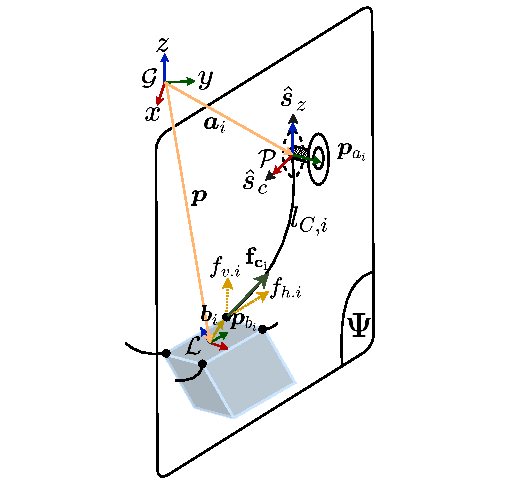
\includegraphics[width=0.6\textwidth]{img/robot_frame.pdf}
	\caption{دیاگرام پنجه ربات متصل به یک کابل  خم‌شده}
	\label{fig:frame_robot}
\end{figure}

ما تغییر شکل کابل را در یک صفحه عمودی دو بعدی $\Psi$ مدل‌سازی می‌کنیم که پولی $\bm{p}_{a_i}$ و نقطه اتصال $\bm{p}_{b_i}$ در پنجه ربات را در بر می‌گیرد. دستگاه‌مختصات
$\mathcal{P}$
روی این صفحه در نقطه $\bm{p}_{a_i}$ قرار دارد و با بردارهای واحد $\hat{\bm{s}}_z$ که موازی با محور $z$ جهانی است و $\hat{\bm{s}}_c$ که در جهت کابل بر روی صفحه $x_{\mathcal{P}}-y_{\mathcal{P}}$  دستگاه‌مختصات $\mathcal{P}$ قرار دارد، تعریف می‌شود.
به طور خاص،  $\hat{\bm{s}}_c = \frac{\bm{b}_{xy_i} - \bm{a}_{xy_i}}{\|\bm{b}_{xy_i} - \bm{a}_{xy_i}\|}$، که در آن $\bm{b}_{xy_i}$ و $\bm{a}_{xy_i}$ به ترتیب اجزای $x-y$ بردارهای $\bm{b}_{i}$ و $\bm{a}_{i}$ در دستگاه‌مختصات جهانی هستند.

\section{معادلات مدل کابل خم‌شده} \label{seq:modeling}

معادلات زنجیره‌ای اثر خم شدن کابل غیرقابل ارتجاع با جرم غیر قابل اغماض را همانطور که در~\cite{pott2013cable} توصیف شده است، به صورت زیر است:

\begin{equation} \label{eq:z(cx)}
	z_i(x_c) = \frac{f_{h,i}}{g_c} \cdot \left( \cosh \left( \frac{g_c}{f_{h,i}} \cdot (x_c + C_{1,i}) \right) - C_{2,i} \right)
\end{equation} 

در این معادله، شکل خم شدن کابل با تابع $z_i(x_c)$ تعریف شده است. ثابت‌های زنجیره‌ای، $C_{1,i}$ و $C_{2,i}$ با توجه به شرایط مرزی نقطه انتهایی $z_i(0)=(\bm{p}_{a})_z$ و $z'_i(L_i)=-\frac{f_v}{f_h}$ تعیین می‌شوند، که در آن $z'_i(L_i)$ شیب معادله (\ref{eq:z(cx)}) در \(x_c = L_i = \|(\bm{b})_{xy_i} - (\bm{a})_{xy_i}\|\) است و به صورت زیر دارای ‌حل بسته هستند:

\begin{equation}  \label{eq:C1}
	C_{1,i} = \frac{f_{h,i}}{g_c} \cdot \operatorname{asinh} \left( \frac{-f_{v,i}}{f_{h,i}} \right) - L_i  
\end{equation}

\begin{equation}  \label{eq:C2}
	C_{2,i} = \cosh \left(C_{1,i} \cdot \frac{g_c}{f_{h,i}} \right) - \frac{g_c}{f_{h,i}} \cdot (\bm{p}_a)_z
\end{equation}

همانطور که در شکل~\ref{fig:frame_robot} نشان داده شده است، $f_{h,i}$ و $f_{v,i}$ اجزای افقی و عمودی نیروی کابل $\mathbf{f}_{c_i}$ در دستگاه‌مختصات $\mathcal{P}$ هستند. علاوه بر این، $g_c=g.\rho_c$ است که در آن $g$ و $\rho_c$ به ترتیب شتاب گرانشی و جرم در واحد طول کابل هستند. در نهایت، طول منحنی معادله (\ref{eq:z(cx)}) به عنوان طول واقعی کابل $l_{C,i}$ تعریف می‌شود و به صورت زیر محاسبه می‌شود:

\begin{equation}  \label{eq:lcat}
	\begin{aligned}
		l_{C,i} &= \int_0^{L_i} \sqrt{1 + \left(\frac{dz}{dx}\right)^2} \, dx \\ &= \frac{f_{h,i}}{g_c} \cdot \left( \sinh \left( \frac{g_c}{f_{h,i}} (L_i + C_{1,i}) \right) - \sinh \left( \frac{g_c}{f_{h,i}} \cdot C_{1,i} \right) \right) 
	\end{aligned}
\end{equation}


\section{سینماتیک ربات}   
تحلیل سینماتیکی یک ربات موازی کابلی فروتحریک شامل هر دو معادلات هندسی و استاتیکی آن است، که به طور معروف به تحلیل سینماتیک-استاتیک معروف است~\cite{carricato2013direct}. نیروی پیچشی
\footnote{wrench}
 پنجه ربات
 $\mathbf{w}_{ee} \in \mathbb{R}^6$ 
به نیروهای کابل $\mathbf{f}_c \in \mathbb{R}^4 $ از طریق ماتریس ژاکوبی $\bm{J} \in \mathbb{R}^{4\times6}$ مرتبط می‌شود:
\begin{equation} \label{eq:static}
	\mathbf{w}_{ee} = \bm{J}^T \mathbf{f}_{c}  
\end{equation}


در این اینجا، فرض می‌کنیم که $\mathbf{w}_{ee}$ تنها توسط گرانش ایجاد شده است و به صورت زیر محاسبه می‌شود:
\begin{equation} \label{eq:example}
	\mathbf{w}_{ee} = m_{e}g \begin{bmatrix} \hat{\bm{s}}_z \\ \bm{b}_{\text{com}} \times \hat{\bm{s}}_z \end{bmatrix}
\end{equation}

که در آن $m_e$ جرم پنجه ربات و $\bm{b}_{com}$ جابجایی بین مبدا دستگاه‌مختصات $\mathcal{L}$ و مرکز جرم (CoM) انتهای ربات است. 
برای پیوند دادن این معادلات استاتیکی با مدل زنجیره‌ای در معادله \eqref{eq:lcat}، هر جزء نیروی کابل به عنوان یک جفت افقی و عمودی نمایش داده می‌شود:  
\begin{equation}
	\mathbf{f}_{c_{i}}= \begin{bmatrix} f_{h,i} & f_{v,i} \end{bmatrix} ^T 
\end{equation}

برای هر $\mathbf{f}_{c_{i}}$، ستون $i^{ام}$ مربوطه از ماتریس ژاکوبی $\bm{J}^T$ به صورت زیر بیان می‌شود:
\begin{equation}
	\bm{J}^T_i= \begin{bmatrix} -\hat{\bm{s}}_{c,i} & \hat{\bm{s}}_{z} \\ -\bm{R}\bm{b}_{i} \times \hat{\bm{s}}_{c,i} & \bm{R}\bm{b}_{i} \times \hat{\bm{s}}_{z}  \end{bmatrix}
\end{equation}

که در آن، ماتریس چرخش $\bm{R}$، بردارهای واحد $\hat{\bm{s}}_{c,i}, \hat{\bm{s}}_{z}$، و بردار اتصال پنجه $\bm{b}_i$ در مختصات محلی، در بخش
\ref{subsec:Assm} 
تعریف شده‌اند. توجه داشته باشید که معادلات استاتیکی در 
\ref{eq:static}
 یک مسئله نامعین
 \footnote{underdetermined}
است که در آن تعداد معادلات کمتر از تعداد متغیرها است. همانطور که در \cite{allak2022kinematics} پیشنهاد شده است، ما تمام نیروهای کابل را بر اساس یک کابل مرجع بیان می‌کنیم. همانطور که در بخش~\ref{sec:calib_factor} مشاهده خواهد شد، این انتخاب، تعداد حسگرهای نیرو مورد نیاز را به تنها یک عدد کاهش می‌دهد که برای ما نیز از اهمیت بالایی برخودار است. همانطور که در~\cite{borgstrom2009nims, allak2022kinematics} ارائه شده است، با تقسیم ماتریس ژاکوبین و بردار نیرو، می‌توان
 \ref{eq:static} 
 را به صورت زیر نوشت:
\begin{equation} \label{eq:wrench-jac-force}
	\mathbf{w}_{ee} = \begin{bmatrix} \bm{J}^T_{\text{ref}} & \bm{J}^T_{\text{res}} \end{bmatrix} \cdot \begin{bmatrix} \mathbf{f}_{c_{\text{ref}}} \\ \mathbf{f}_{c_{\text{res}}} \end{bmatrix} 
\end{equation} 

که نتیجه می‌دهد:
\begin{equation} \label{eq:jacobian-distribution}
	\mathbf{w}_{ee} = \bm{J}_{\text{ref}}^T \cdot \mathbf{f}_{c_{\text{ref}}} + \bm{J}_{\text{res}}^T \cdot \mathbf{f}_{c_{\text{res}}} 
\end{equation}

که در آن، $\bm{J}^T_{\text{ref}}$ نمایانگر یک زیرماتریس $6\times2$ شامل دو ستون اول $\bm{J}^T$ است که مربوط به نیروی کابل مرجع $\mathbf{f}_{c_{\text{ref}}}$ است. به دنبال آن، $\bm{J}^T_{\text{res}}$ به عنوان زیرماتریس باقی‌مانده $6\times6$ تعریف می‌شود و $\mathbf{f}_{c_{\text{res}}}$ نمایانگر نیروهای کابل باقی‌مانده است. ما می‌توانیم $\mathbf{f}_{c_{\text{res}}}$ را در معادله~\eqref{eq:jacobian-distribution} به صورت زیر بازنویسی کنیم:

\begin{equation} \label{eq:force_base_cable_one}
	\mathbf{f}_{c_{\text{res}}} = (\bm{J}_{\text{res}}^T)^{-1} \left( \mathbf{w}_{ee} - \bm{J}_{\text{ref}}^T \cdot \mathbf{f}_{c_{\text{ref}}} \right)
\end{equation}

با این فرمول‌بندی، تعداد متغیرها از 8 به 2 کاهش می‌یابد، در حالی که معادلات استاتیکی به‌طور ضمنی در معادله \eqref{eq:static} نهفته می‌شود و نیاز افزودن یک قید جداگانه را حذف می کند~\cite{borgstrom2009nims}.




\section{گراف عامل کالیبراسیون و مکان‌یابی همزمان سینماتیک-استاتیک} \label{sec:calib_factor}

در این بخش، با استفاده از روابط استخراج شده در قسمت قبل، و همچنین فرمول‌بندی سینماتیکی تعریف شده در فصل پیشین، رویکردی با یک فرمول‌بندی یکپارچه ایجاد می‌شود. رویکرد ما یک گراف عامل با گره‌های متغیر
$\bm{X}(k) \in SE(3)$، $l^0_i$، $\bm{p}_{a_i} \in \mathbb{R}^3$، $\Delta\mathcal{\bm{R}}(k) \in SO(3)$، و $f^{ref}_{h}(k), \ f^{ref}_{v}(k) \in \mathbb{R}$
تعریف می‌کند. این گره‌ها به ترتیب، نمایانگر موقعیت‌های پنجه ربات، مقادیر اولیه طول کابل‌ها، مکان‌های نقاط پولی، و تغییرات در جهت‌گیری ربات، و همچنین نیروی کابل مرجع در محورهای افقی و عمودی در حالت‌های استاتیک ربات هستند. در ساختار فروتحریک ما، همه ترکیب‌های مکانی و جهت‌گیری قابل اجرا نیستند. در اینجا، $\Delta\mathcal{\bm{R}}(k)$ متغیری است که مقدار اولیه چرخش پنجه ربات را تغییر می‌دهد. علاوه بر این، کابل مرجع به عنوان کابلی که کاربر حسگر نیرو برای مقاصد کالیبراسیون بر روی آن تعبیه شده است، تعیین می‌شود.

\begin{figure} [t]
	\centering
	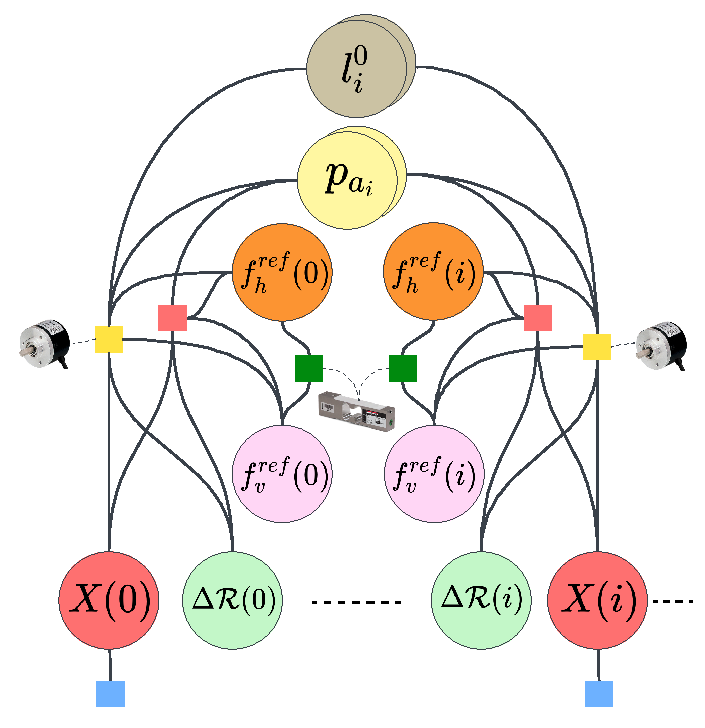
\includegraphics[width=0.55\textwidth]{img/CALIBRATION_GRAPH.pdf}
	\caption{گراف عامل کالیبراسیون و مکان‌یابی همزمان ربات کابلی با کابل‌های خم‌شده}
	\label{fig:calibration_FG}
\end{figure}

شکل~\ref{fig:calibration_FG} ساختار این گراف عامل در راستای کالیبراسیون خودکار و همچنین مکان‌یابی همزمان برای ساختار تعریف شده را که برای دو نمونه از وضعیت‌های استاتیک $0$ و $i$ نمایش داده شده است، نشان می‌دهد. متغیرهای بهینه‌سازی در این گراف با دایره‌های برچسب‌خورده با نام‌های پارامتر‌ها در رنگ‌های مختلف نمایان شده‌اند.
علاوه بر این، عامل‌ها با مربع‌های رنگی به تصویر کشیده شده‌اند، که عامل انکودر و یا همان طول کابل خم‌شده به رنگ زرد، عامل مکان اتصال کابل به پولی به رنگ قرمز، عامل اندازه‌گیری نیرو به رنگ سبز، و عامل پیشین موقعیت به رنگ آبی است. هر عامل بر اساس معادلات سینماتیک و مدل ریاضی تعریف شده برای کابل توصیف‌شده در بخش~\ref{sec:modeling} فرمول‌بندی شده و به شرح زیر تعریف می‌شوند:

\subsection{عامل طول کابل خم‌شده}
این عامل رابطه‌ای بین اندازه‌گیری‌های انکودر و طول واقعی کابل از معادله
\ref{eq:lcat}
 ایجاد می‌کند. این قید اندازه‌گیری برای کابل $i^{ام}$ به صورت زیر فرمول‌بندی می‌شود:
\begin{equation}
	f(z^{enc}_{i}, \bm{\zeta})[k] = l_{C,i}[k] + l^0_i - z^{enc}_{i}[k]
\end{equation}

که در آن $l_{C,i}$ نمایانگر طول واقعی کابل در اثر خم‌شدگی از نیروی وزن آن  به‌طوریکه در معادله~\ref{eq:lcat} تعریف شده است، می‌باشد. همچنین $l^0_i$ نشان‌دهنده مقدار طول اولیه کابل است، و $z^{enc}_{i}$ نمایانگر اندازه‌گیری نسبی انکودر مربوط به کابل $i^{ام}$ است. علاوه بر این، $k$ بیان‌کننده شاخص نمونه داده‌های زمانی است.

\subsection{عامل مکان اتصال کابل به پولی}
این عامل تضمین می‌کند که ارتفاع محاسبه‌شده نقطه اتصال کابل روی پنجه ربات، که از وضعیت پنجه ربات استنتاج شده، با ارتفاع کابل خم‌شده پیش‌بینی‌شده از پولی مربوطه مطابقت داشته باشد. تابع خطا برای پولی $i^{ام}$ به صورت زیر بیان می‌شود:
\begin{equation}
	f(\bm{\zeta})[k] = (p_{b,i})_z [k] - z_i(L_i)[k]
\end{equation}
که در آن، $(p_{b,i})_z$ به ارتفاع نقطه اتصال کابل $i^{ام}$ در مختصات جهانی اشاره دارد، و $z_i(L_i)$ نمایانگر شکل خم‌شدگی کابل در $L_i$ به‌طوریکه در معادله~\ref{eq:z(cx)} توصیف شده است.

\subsection{عامل اندازه‌گیری نیرو}
این عامل نرم نیروی افقی و عمودی را به‌گونه‌ای محدود می‌کند که نزدیک به اندازه‌گیری نیرو از حسگر تعبیه‌شده روی کابل مرجع، در نزدیکی پنجه ربات باشد. توجه داشته باشید که این محدودیت تنها برای کابل مرجع با یک تابع هزینه به صورت زیر مورد نیاز است:
\begin{equation}
	f(f^{m}, \bm{\zeta})[k] = \| [f^{ref}_{h}[k]~~f^{ref}_{v}[k]]^T \| - f^{m}[k]
\end{equation}
در اینجا، $f^{ref}_{h}$ و $f^{ref}_{v}$ به ترتیب نمایانگر نیروهای مرجع کابل در جهت‌های افقی و عمودی هستند، $\|.\|$ نشان‌دهنده نرم اقلیدسی است، و $f^{m}$ مقدار  نیروی کابل مرجع است که توسط حسگر نیرو اندازه‌گیری شده است.

\subsection{عامل پیشین مکان}
عوامل انکودر و اندازه‌گیری نیرو با گره‌های متغیر مکان $\bm{X}(k)$ مرتبط هستند که نمایانگر وضعیت‌های استاتیک ربات در فرآیند کالیبراسیون به‌طوریکه توسط یک سیستم محلی‌سازی مبتنی بر بینایی اندازه‌گیری شده است. 
هر موقعیت به حالات تعادلی مربوط می‌شود که در آن ربات از طریق چهار کابل خود ثابت است. نمونه‌هایی از وضعیت‌های استاتیک در شکل~\ref{fig:calibration_FG} با نشانگرهای $0$ و $i$ برچسب‌گذاری شده‌اند. این عامل پیشین  مکان نیز برای تعریف صفر ربات مورد استفاده قرار می‌گیرد.

























\section{نتایج تجربی} \label{sec:results}
این بخش به منظور اعتبارسنجی مدل و روش کالیبراسیون پیشنهادی از طریق شبیه‌سازی اجزای محدود (FE) سیستم ارائه شده است. ابتدا اعتبار فرمولاسیون‌های کینتواستاتیک بررسی می‌شود و سپس نتایج کالیبراسیون برای دو ربات کابلی کوچک و بزرگ مقیاس نشان داده می‌شود. برای شبیه‌سازی‌های FE از نرم‌افزار RecurDyn~\cite{functionbay} استفاده کردیم، مدل گراف عاملی خود را با استفاده از کتابخانه GTSAM~\cite{dellaert2012factor} پیاده‌سازی کردیم و از SymForce~\cite{Martiros-RSS-22} برای استخراج عوامل و جاکوبین‌های مربوطه استفاده نمودیم.

\begin{figure} [t]
	\centering
	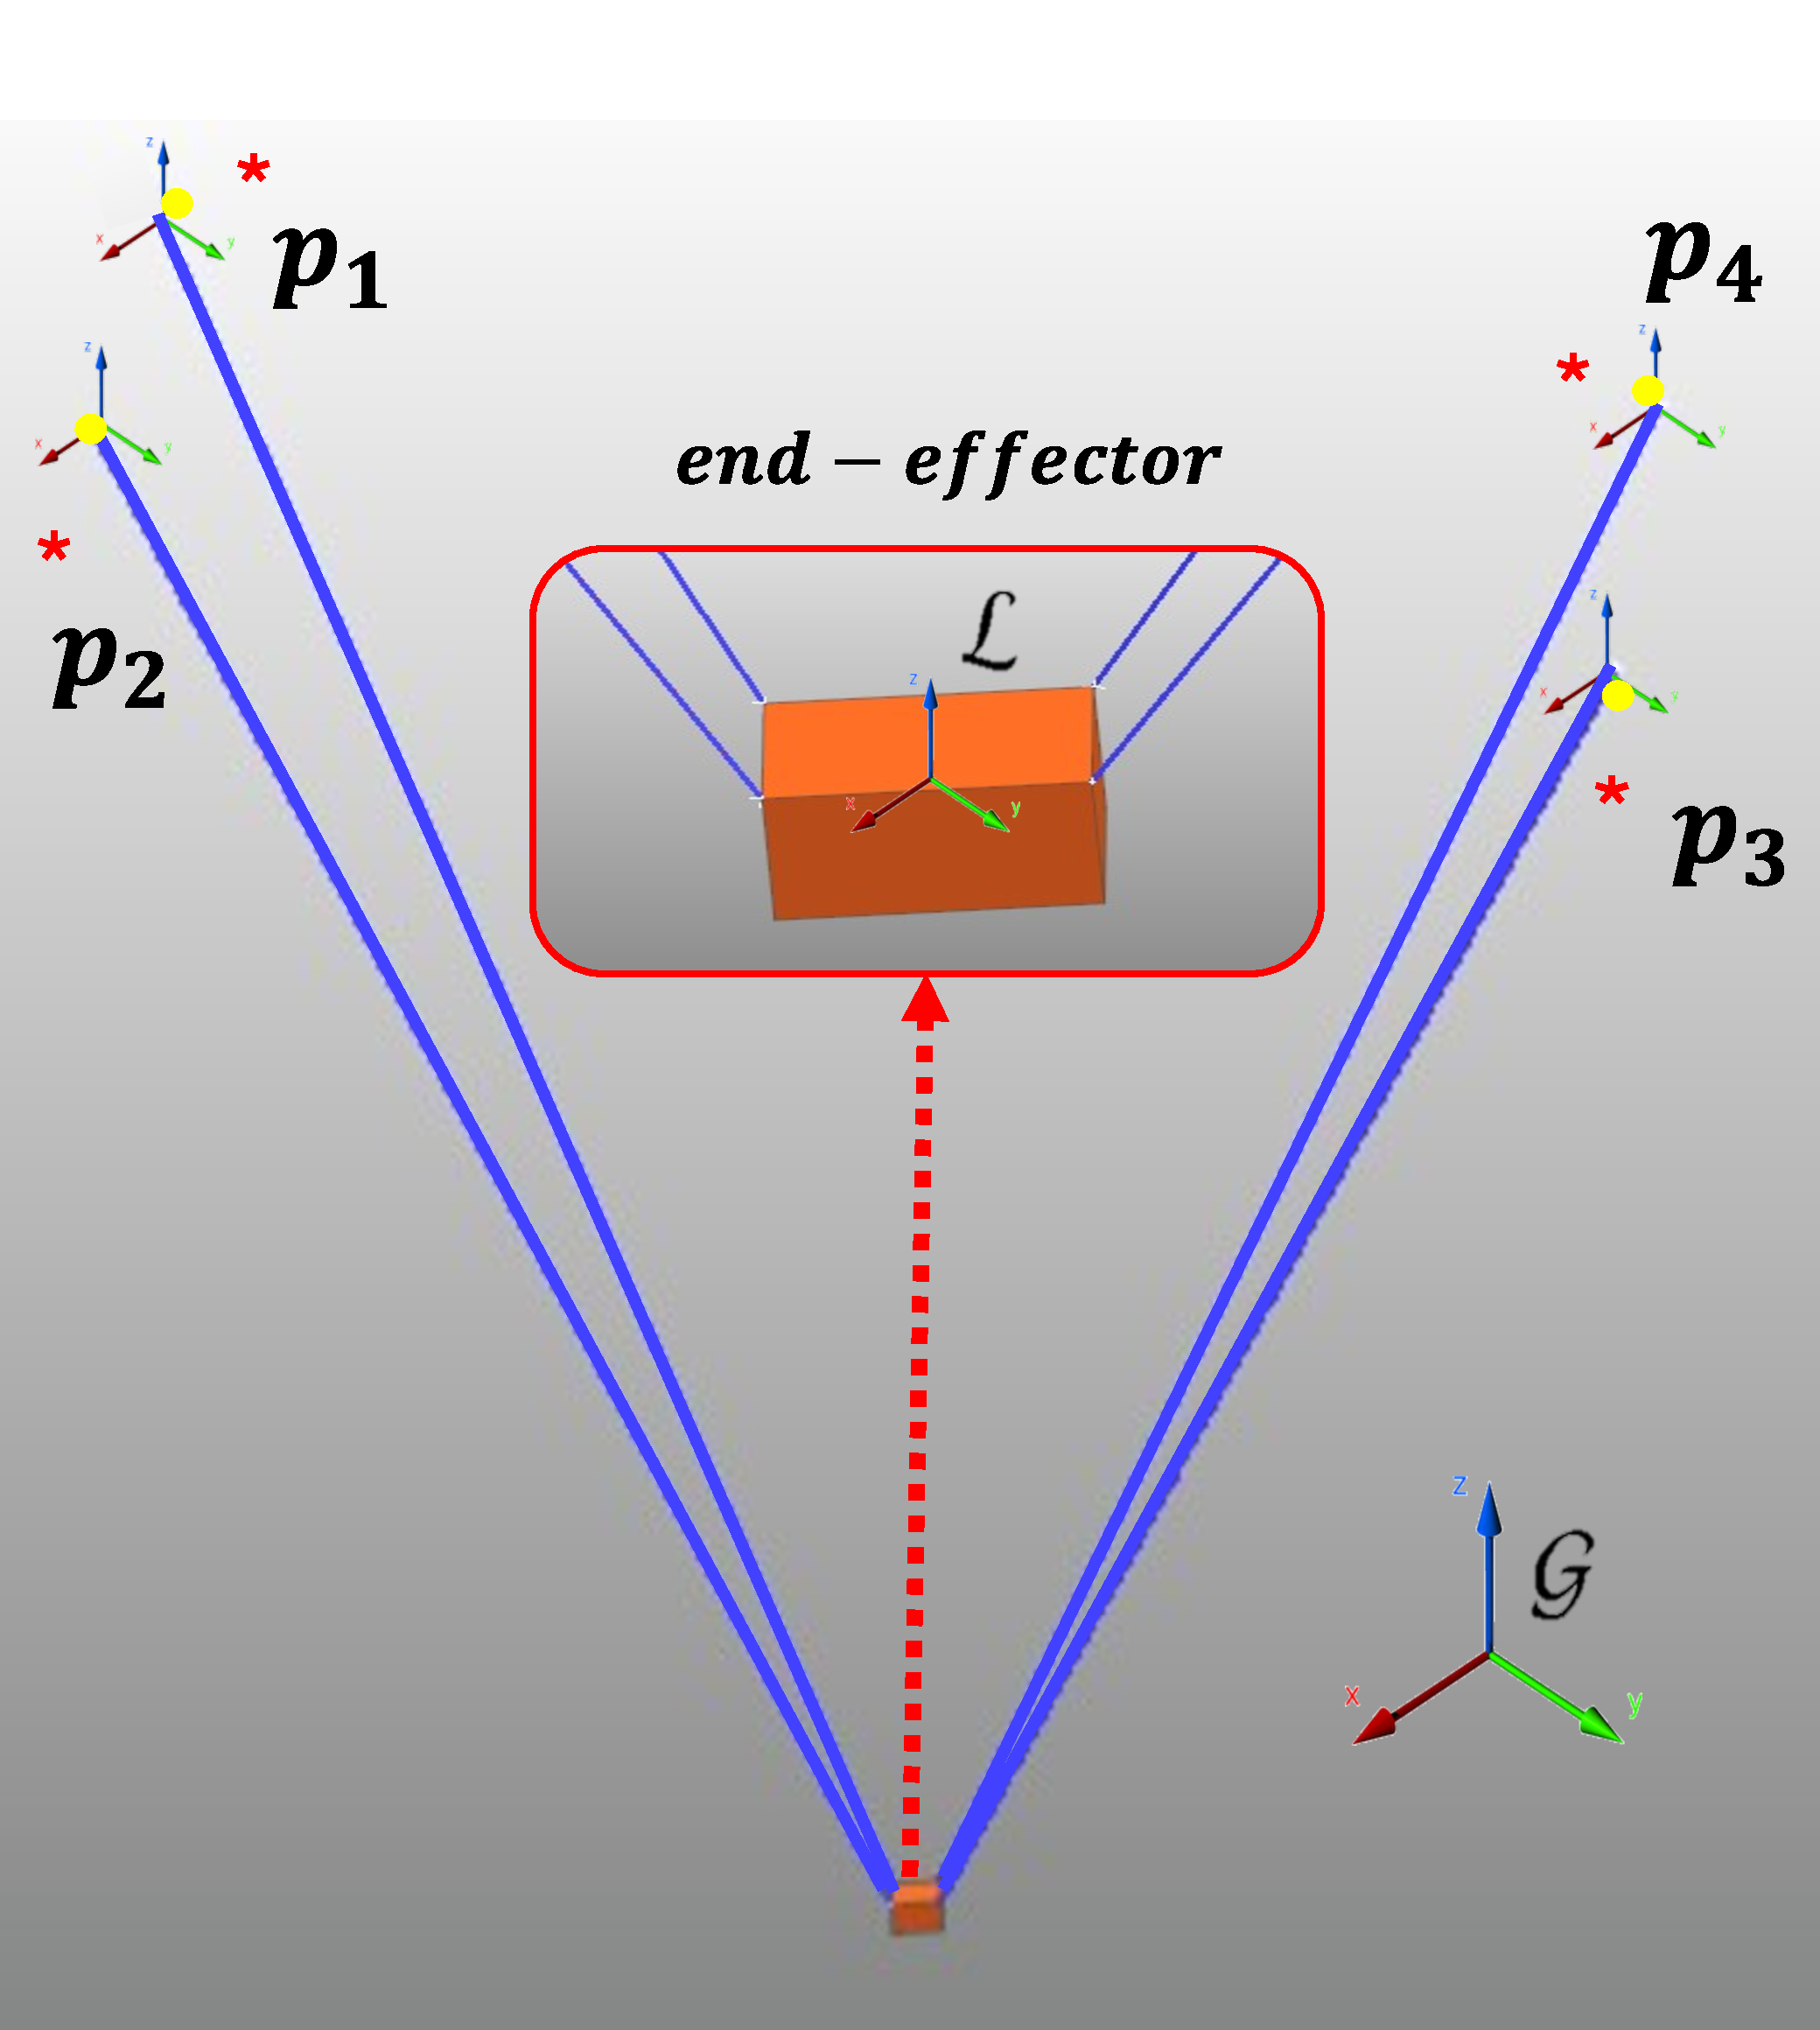
\includegraphics[width=0.25\textwidth]{img/E2_small.pdf}
	\caption{سناریوی ربات کوچک‌مقیاس در محیط شبیه‌ساز RecurDyn}
	\label{fig:recurdyn_small}
\end{figure}

\begin{figure} [b]
	\centering
	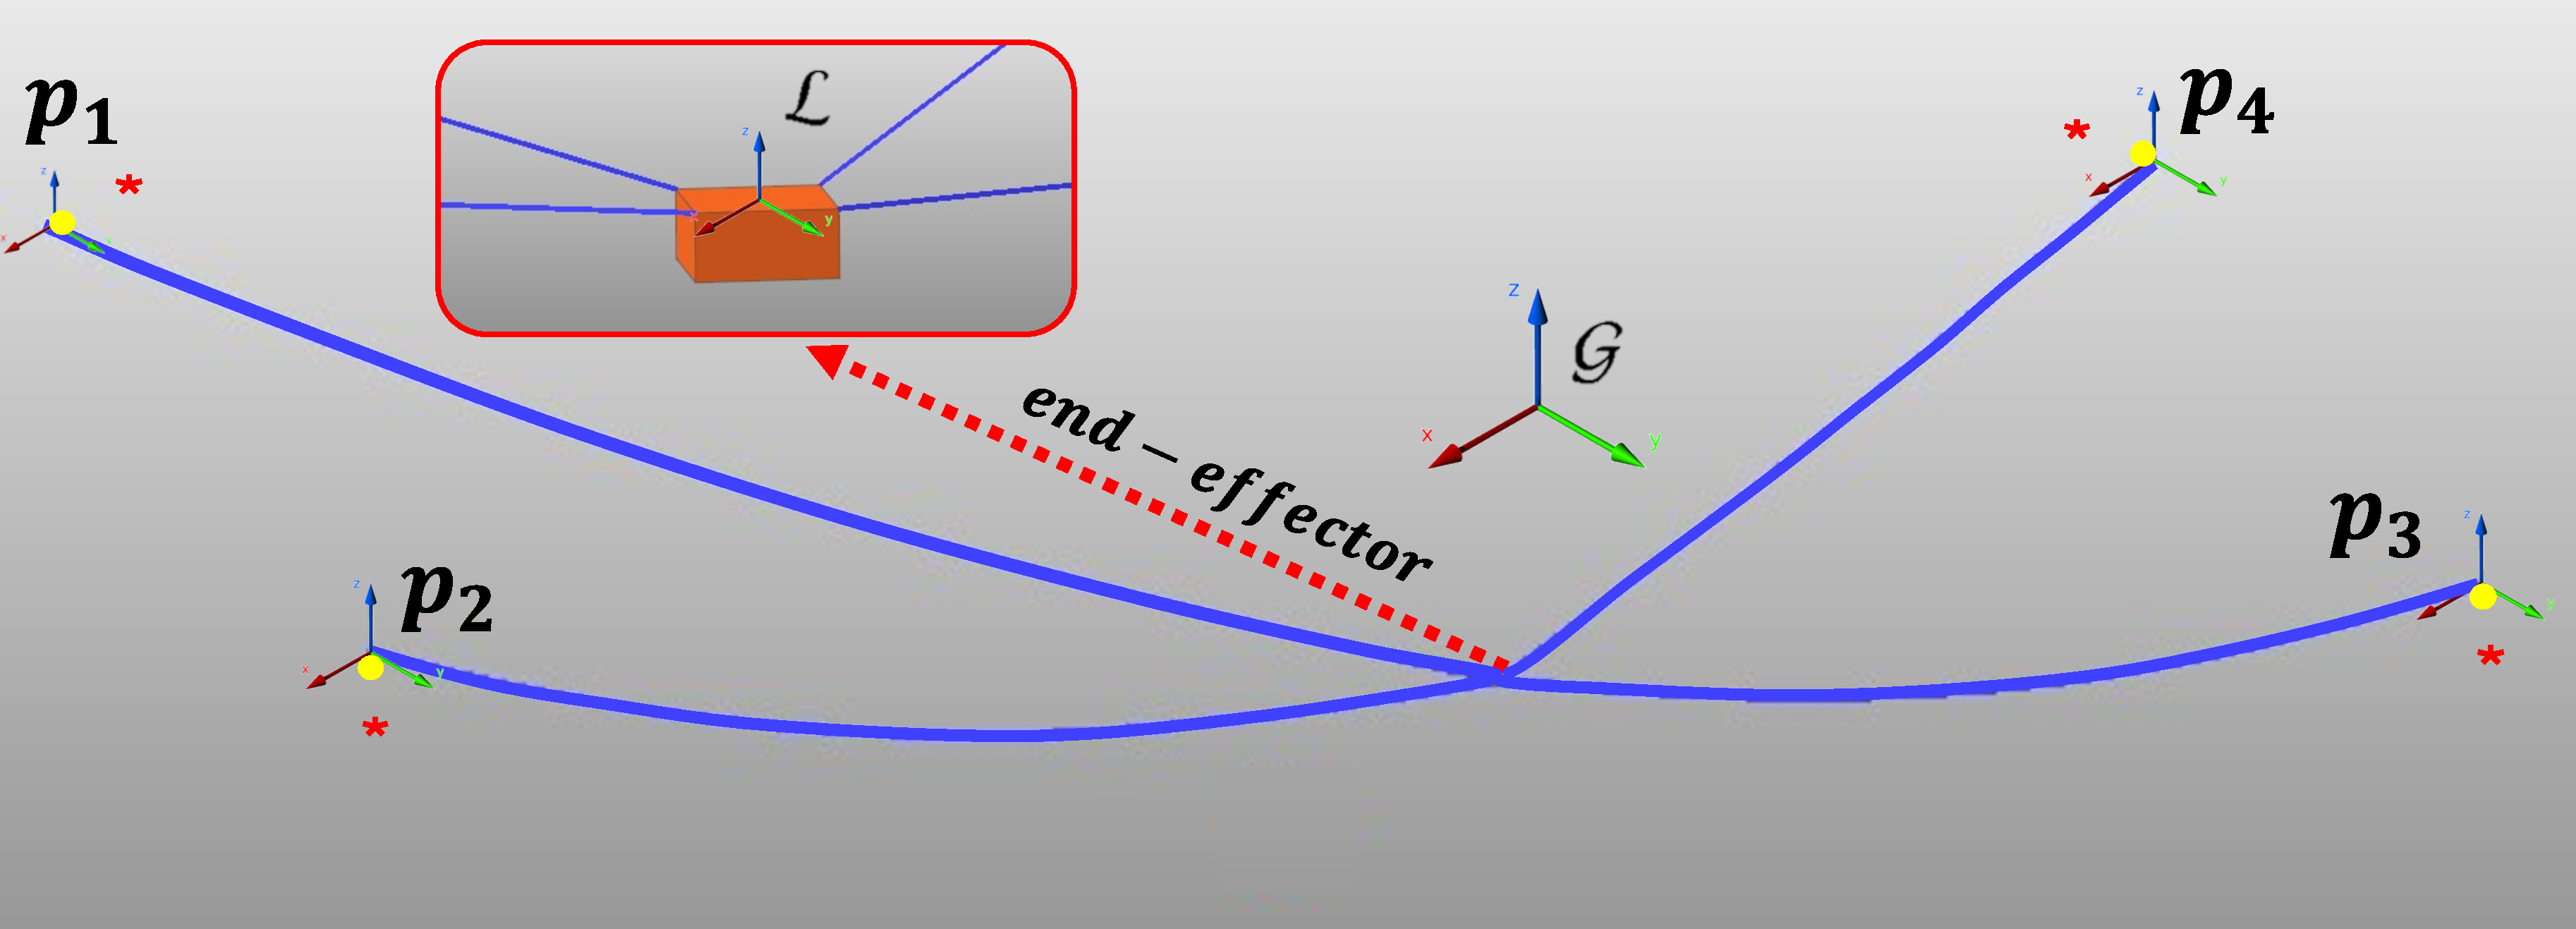
\includegraphics[width=0.46\textwidth]{img/E1_large.pdf}
	\caption{سناریوی ربات بزرگ‌مقیاس در محیط شبیه‌ساز RecurDyn}
	\label{fig:recurdyn_large}
\end{figure}

\subsection{تأیید مدل}
برای تأیید دقت مدل کینتواستاتیک ما، همان‌طور که در بخش \ref{sec:modeling} توضیح داده شده است، گراف عاملی کینتواستاتیک کالیبره شده را با استفاده از عوامل پیشین بر روی متغیرهای استخراج شده از شبیه‌ساز محدود کردیم. دو سناریوی ربات کابلی معلق کوچک و بزرگ مقیاس را تنظیم کردیم. شکل~\ref{fig:recurdyn_small} و شکل~\ref{fig:recurdyn_large} این سناریوهای ربات‌ها را در محیط شبیه‌ساز RecurDyn نشان می‌دهند. هر دو ربات چهار کابل را به چهار گوشه بالای یک جعبه مستطیلی با ابعاد $(12.5, 4.5, 28.5)$ متر برای ربات کوچک و $(240, 220, 50)$ متر برای ربات بزرگ‌تر متصل کرده‌اند، همان‌طور که در جدول~\ref{tab:Model_verification} ذکر شده است. جرم ابزار پایان برای ربات بزرگ به $34 \text{ Kg}$ و برای ربات کوچک به $4.4 \text{ Kg}$ تنظیم شده است. چگالی طول کابل‌ها برای ربات کوچک $10.2 \text{ g/m}$ و برای ربات بزرگ‌تر $72.4 \text{ g/m}$ است، که به نسبت جرم ابزار پایان به کابل به $4.14$ برای ربات کوچک و $0.62$ برای ربات بزرگ‌تر ترجمه می‌شود. همان‌طور که در~\cite{pott2013cable} پیشنهاد شده است، این شرایط نشان‌دهنده تأثیر قابل توجه آویزان شدن برای ربات بزرگ‌تر است.

دو ردیف اول جدول~\ref{tab:Model_verification} درصد خطاهای میانگین در طول کابل پیش‌بینی شده (MPE-L) و نیرو (MPE-F) محاسبه شده در 5 موقعیت ایستای تصادفی را ارائه می‌دهد. این مقادیر نشان می‌دهند که تطابق نزدیکی بین نیروی کابل و مقادیر طول کابل کاتناری محاسبه شده از مدل ریاضی ما و مقادیر مربوطه از شبیه‌ساز وجود دارد. به طور خاص، برای ربات بزرگ مقیاس، MPE-L و MPE-F به ترتیب برابر با $\%0.0089$ و $\%0.9154$ ارزیابی شده است، که بسیار کوچک‌تر از دامنه‌های طول کابل و نیرو برای هر ربات است، همان‌طور که در جدول نیز ارائه شده است. همان‌طور که به طور شهودی انتظار می‌رود، این تطابق برای ربات کابلی کوچک‌تر دقیق‌تر است، که طول کابل و نیروهای پیش‌بینی شده در ستون سوم این جدول نشان داده شده است.

\begin{table}[t]
	\centering
	\caption{Model Verification}
	\label{tab:Model_verification}
	\renewcommand{\arraystretch}{1.45} % Increase row spacing
	\footnotesize
	\begin{tabular}{c|c|c}
		\toprule
		\rowcolor{gray!10}
		\hline
		\text{Scenario} & \text{Large scale} & \text{Small scale} \\
		\midrule
		MPE-L (\%) & 8.8947$\times10^{-3}$ & 7.3595$\times10^{-3}$ \\
		\hline
		MPE-F (\%) & 0.9154 & 0.9046 \\
		\hline
		$[l_{\min}, l_{\max}]$ (m)& $[134.7, 200.7]$ & $[10.8, 25.9]$ \\
		\hline
		$[f_{\min}, f_{\max}]$ (N)& $[489.1, 954.3]$ & $[12.4, 26.2]$ \\
		\hline
		Pulley configuration ($\text{m}^3$) & $240\times220\times50 $ & $12.5\times 4.5 \times 28.5$ \\
		\hline
		End-effector mass ($\text{Kg}$) & $34.0$ & $4.4$ \\
		\hline
		\multirow{2}{*}{Cable properties} & \multirow{2}{*}{\begin{tabular}[c]{@{}c@{}} $\rho = 1.44~~(\text{g}/\text{cm}^2)$ \\ $\text{radius} = 4.0~~(\text{mm})$ \end{tabular}} & \multirow{2}{*}{\begin{tabular}[c]{@{}c@{}} $\rho = 1.44~~(\text{g}/\text{cm}^2)$ \\ $\text{radius} = 1.5~~(\text{mm})$  \end{tabular}} \\
		& & \\
		\bottomrule
	\end{tabular}
\end{table}


\subsection{کالیبراسیون}
در این بخش، ما روش کالیبراسیونی را که در این مقاله پیشنهاد شده است، همان‌طور که در بخش~\ref{sec:calibration_factor_graph} توضیح داده شده است، پیاده‌سازی می‌کنیم و اهمیت مدل‌سازی آویزان شدن کابل را از طریق نتایج شبیه‌سازی نشان می‌دهیم. علاوه بر این، به طور خلاصه به مسئله مقداردهی اولیه کالیبراسیون پرداخته و یک راه‌حل احتمالی را پیشنهاد می‌کنیم.

\subsubsection{کالیبراسیون با آویزان شدن کابل}
هدف ما در فرآیند کالیبراسیون کینماتیکی، تعیین مکان‌های نقطه‌های لنگر و جابجایی‌های کدور کابل طول با استفاده از اندازه‌گیری‌های مجموعه‌ای از وضعیت‌های ابزار پایان، اندازه‌گیری‌های طول نسبی کابل و تنها مقادیر کشش کابل مرجع در نقطه اتصال ابزار پایان است. طبق آزمایشات ما، بسیار مهم است که توزیع نمونه‌ها به طور جامع دامنه وضعیت ربات را پوشش دهد. توسعه نسل‌های تحلیلی و آگاه به مشاهده برای پرداختن به این مشکل شناسایی موضوع تحقیق آینده است.

ما داده‌های حسگر شبیه‌سازی شده خود را از نرم‌افزار RecurDyn دریافت کردیم و تغییرات نویز گاوسی صفر میانگین را برای وارد کردن نویز پیش‌بینی‌شده حسگر معرفی کردیم. به ویژه، ما انحراف استاندارد $10mm$ برای طول کابل، $5N$ برای حسگر نیرو در ربات بزرگ‌مقیاس و $1N$ برای حسگر ربات کوچک‌مقیاس اعمال کردیم. وضعیت‌های ابزار پایان با $\Delta \mathbf{T} = \exp(\hat{\boldsymbol{\xi}})$ که در آن $\hat{\boldsymbol{\xi}} \in \mathfrak{se}(3)$ عنصر جبر لی متناظر با بردار پیچ $\boldsymbol{\xi} \in \mathbb{R}^6$ است، دچار تغییر شد. این بردارهای پیچ تغییرات از توزیع گاوسی صفر میانگین $\boldsymbol{\xi}\sim\mathcal{N}(\mathbf{0}, \boldsymbol{\Sigma})$ با ماتریس کوواریانس $\boldsymbol{\Sigma}$ انتخاب شده با انحراف $0.005$ متر در ترجمه و $0.01$ رادیان در درجات آزادی چرخشی نمونه‌برداری شدند.
برای مقداردهی اولیه گراف عاملی، مکان‌های نقطه‌های لنگر واقعیت‌سنجی را با دامنه $1$ متر برای ربات کوچک و $10$ متر برای پلتفرم بزرگ دچار تغییر کردیم. علاوه بر این، این تغییرات برای جابجایی‌های اولیه کابل به $10$ متر و $80$ متر برای ربات کوچک و بزرگ، به ترتیب، تنظیم شد. ما تخمین اولیه برای نیروی کابل مرجع در محور عمودی را به عنوان $f^{{ref}}_{v_0}=m_eg/4$ در نظر گرفتیم و برای محور افقی به صورت زیر:
\begin{equation}  \label{eq:fh_0}
	f^{ref}_{h_0}=\frac{f^{{ref}}_{v_0}}{\tan(\alpha)} 
\end{equation}
که در آن $\alpha$ به صورت زیر تعریف می‌شود:
\begin{equation}  \label{eq:alpha}
	\alpha = \arccos\left(\frac{\hat{\bm{s}}_{c_{ref}}^T \cdot [\bm{p}_{b_{\text{ref}}} - \bm{p}_{a_{\text{ref}}}]}{\| \bm{p}_{b_{\text{ref}}} - \bm{p}_{a_{\text{ref}}} \|}\right)
\end{equation}
در این زمینه، $\hat{\bm{s}}_{c_{ref}}$ بردار واحدی است که در بخش \ref{sec:modeling} تعریف شده است و از تخمین‌های اولیه موقعیت قرقره استفاده می‌کند. مهم است که این نقاط به لنگرهای مربوط به کابل مرجع مربوط می‌شوند.

نتایج کالیبراسیون برای مکان‌های لنگر و جابجایی‌های طول کابل در جدول~\ref{tab:calibration_results} ارائه شده است. این نتایج مربوط به سناریوهای نشان داده شده در شکل~\ref{fig:recurdyn_small} و شکل~\ref{fig:recurdyn_large} است، که در آن مکان‌های لنگر اولیه با ستاره‌های قرمز و مکان‌های لنگر کالیبره شده با دایره‌های زرد برای هر دو مورد نشان داده شده است.
در این جدول، سه سناریوی مختلف کالیبراسیون برای ربات بزرگ‌مقیاس با تعداد مختلف نقاط نمونه‌برداری شده برای روتین بهینه‌سازی گزارش شده است. همان‌طور که انتظار می‌رود، دقت کالیبراسیون با افزایش تعداد نقاط نمونه‌برداری بهبود می‌یابد و نتایج دقیق‌تری را با 35 نمونه داده برای ربات بزرگ و 8 موقعیت نمونه برای ربات کوچک ارائه می‌دهد. ما معتقدیم که برای ربات بزرگ‌تر، پارامترهای مربوط به آویزان شدن کابل تأثیر عمیق‌تری بر دقت کالیبراسیون دارند. این در نوبه خود تعداد مؤثر پارامترهای مدل را افزایش می‌دهد و نیاز به نقاط نمونه‌برداری بیشتری برای شناسایی مناسب دارد.

\begin{table}[!t]
	\small
	\centering
	\caption{Calibration Results with Proposed Algorithm}
	\label{tab:calibration_results}
	\renewcommand{\arraystretch}{1.45} % Increase row spacing Me?
	\footnotesize
	\begin{tabular}{c|c|c|c|c}
		\toprule
		\rowcolor{gray!10}
		\hline
		\diagbox[width=2.4cm, height=1.1cm]{MAE (m)}{Scenario} & \multicolumn{1}{c|}{\begin{tabular}[c]{@{}c@{}}large \\ (9 poses)\end{tabular}} & \multicolumn{1}{c|}{\begin{tabular}[c]{@{}c@{}}large \\ (18 poses)\end{tabular}} & \multicolumn{1}{c|}{\begin{tabular}[c]{@{}c@{}}large \\ (35 poses)\end{tabular}} & \multicolumn{1}{c}{\begin{tabular}[c]{@{}c@{}}short \\ (8 poses)\end{tabular}} \\
		\midrule
		$\text{Pulley}_\text{Avg.}$ &  0.387 &  0.226  &   0.191  &   0.149 \\
		\hline
		$\text{Offset}_\text{Avg.}$ &  0.380  &  0.217  &   0.173  &   0.115 \\
		\bottomrule
	\end{tabular}
\end{table}

\section{بحث} \label{sec:discussion}

\subsection{اهمیت در نظر گرفتن اثر آویزان شدن کابل}
برای بررسی اهمیت در نظر گرفتن اثر آویزان شدن کابل، ما فرآیند کالیبراسیون را برای ربات بزرگ‌تر با استفاده از گراف عاملی ساده‌سازی شده که مدل کابل بی‌وزن جامد را استفاده می‌کند، همان‌طور که در~\cite{khorrambakht2023graph} گزارش شده است، انجام دادیم. در نتیجه، به دلیل این ساده‌سازی، خطای میانگین مطلق به طور قابل توجهی از $0.19$ به $2.34$ متر افزایش یافته است که نشان‌دهنده کاهش قابل توجهی در دقت کالیبراسیون است. این تفاوت قابل توجه در کیفیت کالیبراسیون اهمیت حیاتی در نظر گرفتن آویزان شدن کابل را تاکید می‌کند.

\subsection{نکات مربوط به روش مقداردهی اولیه}
همان‌طور که در~\cite{khorrambakht2023graph} ذکر شده است، یکی از نگرانی‌های اصلی در حل مسئله بهینه‌سازی کالیبراسیون غیرمقعر و غیرخطی، مقداردهی اولیه صحیح آن است. اگر مقادیر اولیه به اندازه کافی نزدیک به راه‌حل جهانی نباشند، نتیجه ممکن است به شدت منحرف شود یا بهینه‌ساز حتی ممکن است منحرف شود. چارچوب ارائه شده در~\cite{khorrambakht2023graph} تلاش می‌کند تا این مسئله مقداردهی اولیه را با استفاده از خروجی تقریبی یک الگوریتم بهینه‌سازی جهانی مونت کارلو حل کند. با این حال،~\cite{khorrambakht2023graph} مدل کابل جامد بدون اثرات آویزان شدن را فرض می‌کند. ما معتقدیم که این الگوریتم به طور مستقیم می‌تواند برای مقداردهی اولیه مسئله کالیبراسیون توسعه یافته ارائه شده در این مقاله به کار رود. همان‌طور که قبلاً ذکر شد، دقت کالیبراسیون ربات کابل بزرگ با مدل کابل ساده شده $2.34$ متر بود. این مقدار به طور قابل توجهی کوچکتر از تغییرات ما در طول آزمایشات کالیبراسیون ($10$ متر) است. این نشان می‌دهد که ما می‌توانیم با خیال راحت الگوریتم بهینه‌سازی خود را با خروجی‌های الگوریتم مشابهی که در~\cite{khorrambakht2023graph} ارائه شده است، مقداردهی اولیه کنیم. تأیید این فرضیه برای موارد خاص ارائه شده در این مقاله به دلیل محدودیت‌های شبیه‌ساز مورد استفاده برای تولید تصاویر/داده‌های حسگر LiDAR مورد نیاز برای اجرای این الگوریتم امکان‌پذیر نبود. بررسی این ایده با استفاده از شبیه‌سازهای واقع‌گرایانه موضوع تحقیق آینده است.
